\documentclass[tikz,border=5pt]{standalone}
\usepackage{tikz}\n\usepackage{amssymb}
\usepackage{pgfplots}
\pgfplotsset{compat=1.18}
\definecolor{pbdarkblue}{HTML}{1E3A8A}
\definecolor{pbdarkgreen}{HTML}{065F46}
\definecolor{pbdarkred}{HTML}{991B1B}

\begin{document}
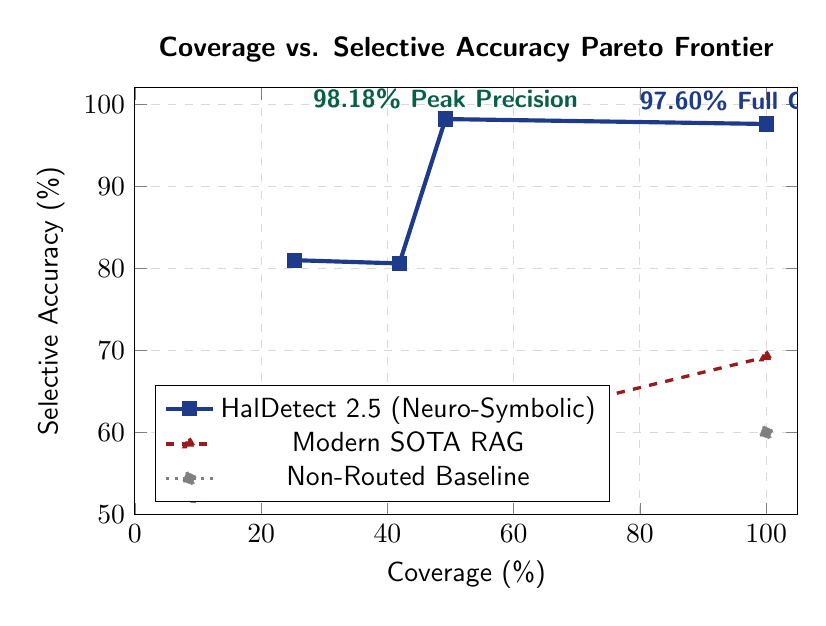
\begin{tikzpicture}
\begin{axis}[
    title={\textbf{Coverage vs. Selective Accuracy Pareto Frontier}},
    xlabel={Coverage (\%)},
    ylabel={Selective Accuracy (\%)},
    xmin=0, xmax=105,
    ymin=50, ymax=102,
    grid=major,
    grid style={dashed, gray!30},
    legend pos=south west,
    width=10cm, height=7cm,
    font=\sffamily
]

% HalDetect Curve
\addplot[
    color=pbdarkblue,
    mark=square*,
    line width=1.5pt
] coordinates {
    (25.3, 81.0)
    (41.9, 80.6)
    (49.2, 98.2)
    (100.0, 97.6)
};
\addlegendentry{HalDetect 2.5 (Neuro-Symbolic)}

% Modern SOTA RAG
\addplot[
    color=pbdarkred,
    mark=triangle*,
    dashed,
    line width=1.2pt
] coordinates {
    (10.0, 52.0)
    (40.0, 58.0)
    (100.0, 69.2)
};
\addlegendentry{Modern SOTA RAG}

% Non-Routed Baseline
\addplot[
    color=gray,
    mark=*,
    dotted,
    line width=1.2pt
] coordinates {
    (100.0, 60.0)
};
\addlegendentry{Non-Routed Baseline}

\node[above, font=\small\sffamily, color=pbdarkgreen] at (axis cs:49.2, 98.2) {\textbf{98.18\% Peak Precision}};
\node[above, font=\small\sffamily, color=pbdarkblue] at (axis cs:100.0, 97.6) {\textbf{97.60\% Full Coverage}};

\end{axis}
\end{tikzpicture}
\end{document}